Funktionen sind im wesentlich Zuordnungen.
\subsection{Begriffe}
\begin{description}
    \item[Definition] Zur Definition einer Funktion $f$ braucht man drei Dinge
    \begin{itemize}
        \item Menge $A$, der Definitionsbereich von $f$, $A = D_f$
        \item Menge $B$, der Wertevorrat von $f$, $B = W_f$
        \item Eine Zuordnung, die jedem $a \in A$ genau ein Element $b \in B$ zuordnet \\
        Schreibweise: $b = f(a)$ bzw. $a \longmapsto f(a)$ \\
        Mathematisch wird diese Zuordnung gegeben durch eine Menge von geordneten Paaren
        $$\textrm{Graph}(f) = \lbrace(a,f(a)) | a \in A \rbrace \subseteq A \times B$$
        mit den Eigenschaften:
        \begin{itemize}
            \item $(\forall a \in A)(\exists b \in B)\ (a;b) \in \textrm{Graph}(f)$ (Vollständigkeit)
            \item $(\forall a \in A)(\forall b_1,b_2 \in B)\ (a;b_1);(a;b_2) \in \textrm{Graph}(f)\Rightarrow b_1 = b_2$ (Eindeutigkeit)
        \end{itemize}
    \end{itemize}
    \item[Schreibweise]
    \begin{alignat*}{3}
        f :\  & A \longrightarrow &  & B \quad , \quad a &  & \longmapsto f(a) = \cdots \\
        & D_f               &  & W_v               &  & \textrm{Graph}
    \end{alignat*}
    \item[Bild] Die Menge aller Funktionswerte von $f$. $\lbrace f(a) | a \in A \rbrace = \lbrace b \in B  | (\exists a \in A) b = f(a) \rbrace \subseteq B$
    \item[surjektiv] $(\forall b \in B)(\exists a \in A) \ f(a) = b$ \\
    \begin{tabularx}{\linewidth}{l|X}
        \adjustbox{valign = t}{
            \begin{tikzpicture}[thick, set/.style = {ellipse, minimum width = 2cm, minimum height = 4cm, draw = black, align = center}, element/.style = {circle, draw = black, minimum size = 0.7, outer sep = 0.05cm}]
                \node [set, label={90:$A$}] (A) at (-1.5,0) {};
                \node [set, label={90:$B$}] (B) at (1.5,0) {};
                \node [element] (1) at (-1.5, 1.5) {1};
                \node [element] (2) at (-1.5, 0.5) {2};
                \node [element] (3) at (-1.5, -0.5) {3};
                \node [element] (4) at (-1.5, -1.5) {4};
                \node [element] (A) at (1.5, 1.5) {A};
                \node [element] (B) at (1.5, 0.5) {B};
                \node [element] (C) at (1.5, -0.5) {C};
                \draw [->] (1) to (A);
                \draw [->] (2) to (B);
                \draw [->] (3) to (C);
                \draw [->] (4) to (C);
            \end{tikzpicture}
        } &
        Für jedes Element in $B$ existiert (mindestens) ein Urbild in $A$. Für jede rein surjektive Abbildung gilt:
        $$|A|>|B|$$ \\ \hline
    \end{tabularx}
    \item[injektiv] $(\forall a_1,a_2 \in A) (a_1 \not = a_2 \Rightarrow f(a_1) \not = f(a_2))$ \\
    \begin{tabularx}{\linewidth}{l|X}
        \adjustbox{valign = t}{
            \begin{tikzpicture}[thick, set/.style = {ellipse, minimum width = 2cm, minimum height = 4cm, draw = black, align = center}, element/.style = {circle, draw = black, minimum size = 0.7, outer sep = 0.05cm}]
                \node [set, label={90:$A$}] (A) at (-1.5,0) {};
                \node [set, label={90:$B$}] (B) at (1.5,0) {};
                \node [element] (1) at (-1.5, 1.5) {1};
                \node [element] (2) at (-1.5, 0.5) {2};
                \node [element] (3) at (-1.5, -0.5) {3};
                \node [element] (A) at (1.5, 1.5) {A};
                \node [element] (B) at (1.5, 0.5) {B};
                \node [element] (C) at (1.5, -0.5) {C};
                \node [element] (D) at (1.5, -1.5) {D};
                \draw [->] (1) to (A);
                \draw [->] (2) to (B);
                \draw [->] (3) to (D);
            \end{tikzpicture}
        } &
        Für jede zwei Elemente in $A$ gilt, dass wenn sie verschieden von einander sind, dann auch ihre Funktionswerte von $f$ verschieden sind. Also hat jedes Element in $B$ höchstens ein Urbild. Für jede rein injektive Abbildung gilt:
        $$|A|<|B|$$ \\ \hline
    \end{tabularx}
    \item[bijektiv]  surjektiv $\wedge$ injektiv: $(\forall b \in B)(\exists ! a \in A)\ f(a) = b$ \\
    \begin{tabularx}{\linewidth}{l|X}
        \adjustbox{valign = t}{
            \begin{tikzpicture}[thick, set/.style = {ellipse, minimum width = 2cm, minimum height = 4cm, draw = black, align = center}, element/.style = {circle, draw = black, minimum size = 0.7, outer sep = 0.05cm}]
                \node [set, label={90:$A$}] (A) at (-1.5,0) {};
                \node [set, label={90:$B$}] (B) at (1.5,0) {};
                \node [element] (1) at (-1.5, 1.5) {1};
                \node [element] (2) at (-1.5, 0.5) {2};
                \node [element] (3) at (-1.5, -0.5) {3};
                \node [element] (4) at (-1.5, -1.5) {4};
                \node [element] (A) at (1.5, 1.5) {A};
                \node [element] (B) at (1.5, 0.5) {B};
                \node [element] (C) at (1.5, -0.5) {C};
                \node [element] (D) at (1.5, -1.5) {D};
                \draw [->] (1) to (A);
                \draw [->] (2) to (B);
                \draw [->] (3) to (C);
                \draw [->] (4) to (D);
            \end{tikzpicture}
        } &
        Für jedes Element in $B$ existiert genau ein Urbild in $A$. Für jede bijektive Abbildung gilt:
        $$|A|=|B|$$ \\ \hline
    \end{tabularx}
    \item[Identitätsfunktion] $id_A : A \longrightarrow A , a \longmapsto a$ z.B. $f(x) = x$
    \item[Komposition] $f : A \longrightarrow B;\ g : B \longrightarrow C$
    $$(g \circ f) : A \longrightarrow C, a \longmapsto g(f(a))$$
    \begin{alignat*}{3}
        f : A \longrightarrow B \Rightarrow & f    &  & = f \circ id_A &  & = id_A \circ f \\
        & f(a) &  & = f(id_A(a))   &  & = id_A(f(a))
    \end{alignat*}
\end{description}
\subsection{Umkehrfunktion}
\begin{description}
    \item[Umkehrbarkeit] (im engeren sinne) $f : A \longrightarrow B$
    $$\leftrightarrow (\exists g : B \longrightarrow A) g \circ f = id_A \wedge f \cdot g = id_B$$
    $$(\forall a \in A)\ g(f(a)) = a$$
    $$(\forall b \in B)\ f(g(b)) = b$$
    Die Funktion $g : B \longrightarrow A$ heißt dann Umkehrfunktion von f, geschrieben $g = f^{-1}$.
    $$f^{-1} \not = (f)^{-1}$$
    Satz: Eine Funktion $f : A \longrightarrow B$ ist genau dann umkehrbar (i.e.s), wenn sie bijektiv ist.
    \item[Umkehrbarkeit in der Analysis] Eine Funktion $f : A \longrightarrow B$ heißt Umkehrbar, wenn die zugehörige Funktion $f : A \longrightarrow \textrm{Bild}(f)$ umkehrbar ist.
    Satz: Eine Funktion $f : A \longrightarrow B$ ist genau dann umkehrbar (i.w.s), wenn sie injektiv ist.
\end{description}
\subsubsection{Potenzfunktion} $$f : \mathbb{R} \longrightarrow \mathbb{R},\ x \longmapsto x^n$$
\begin{description}
    \item[quadratisch] \
    \begin{tabular}[t]{cc}
        $f : \mathbb{R} \longrightarrow \mathbb{R},\ x \longmapsto x^2$ & $f^{*-1} : \mathbb{R}_0^+ \longrightarrow \mathbb{R},\ x \longmapsto \sqrt{x}$ \\
        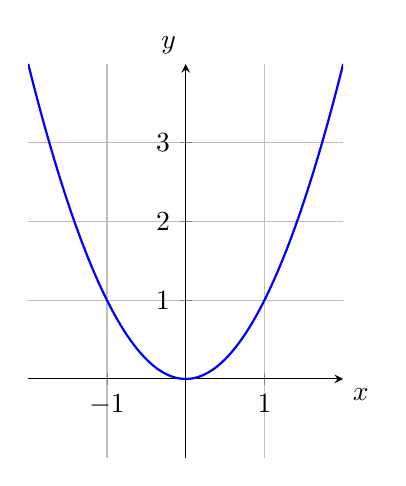
\begin{tikzpicture}
            \begin{axis}[
            x = 1cm, y = 1cm,
            xmin = -2, xmax = 2,
            ymin = -1, ymax = 4,
            axis lines = center,
            xtick={-1,0,...,1},
            ytick={0,1,...,3},
            xlabel={$x$},
            ylabel={$y$},
            xlabel style={below right},
            ylabel style={above left},
            grid=both]
            \addplot[
                domain = -2:2,
                samples = 200,
                smooth,
                thick,
                blue,
            ] {x^2};
            \end{axis}
        \end{tikzpicture}                                      &
        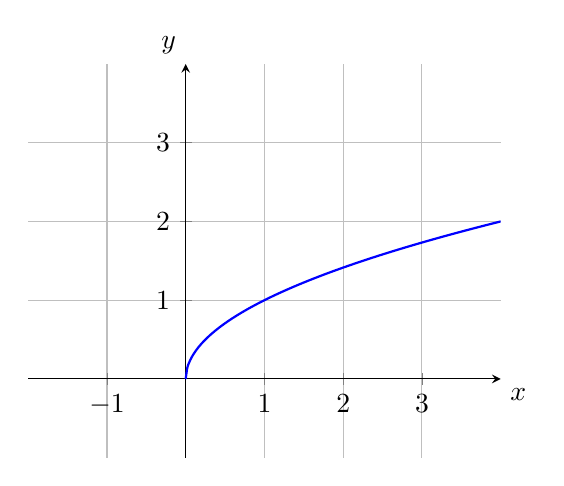
\begin{tikzpicture}
            \begin{axis}[
            x = 1cm, y = 1cm,
            xmin = -2, xmax = 4,
            ymin = -1, ymax = 4,
            axis lines = center,
            xtick={-1,0,...,3},
            ytick={0,1,...,3},
            xlabel={$x$},
            ylabel={$y$},
            xlabel style={below right},
            ylabel style={above left},
            grid=both]
            \addplot[
                domain = 0:4,
                samples = 200,
                smooth,
                thick,
                blue,
            ] {sqrt(x)};
            \end{axis}
        \end{tikzpicture}
    \end{tabular}
    \item[kubisch] \
    \begin{tabular}[t]{cc}
        $f : \mathbb{R} \longrightarrow \mathbb{R},\ x \longmapsto x^3$ & $f^{-1} : \mathbb{R} \longrightarrow \mathbb{R},\ x \longmapsto \sqrt[3]{x}$ \\
        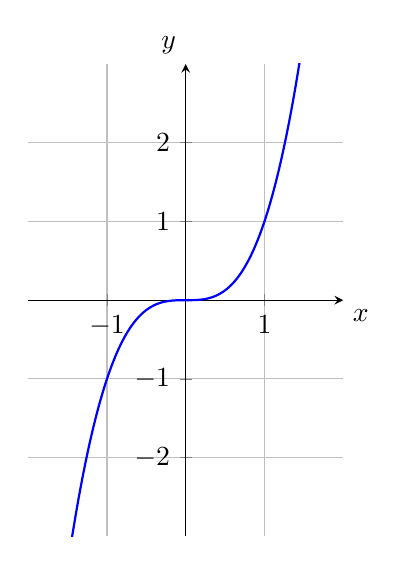
\begin{tikzpicture}
            \begin{axis}[
            x = 1cm, y = 1cm,
            xmin = -2, xmax = 2,
            ymin = -3, ymax = 3,
            axis lines = center,
            xtick={-1,0,...,1},
            ytick={-2,-1,...,2},
            xlabel={$x$},
            ylabel={$y$},
            xlabel style={below right},
            ylabel style={above left},
            grid=both]
            \addplot[
                domain = -2:2,
                samples = 200,
                smooth,
                thick,
                blue,
            ] {x^3};
            \end{axis}
        \end{tikzpicture}                                      &
        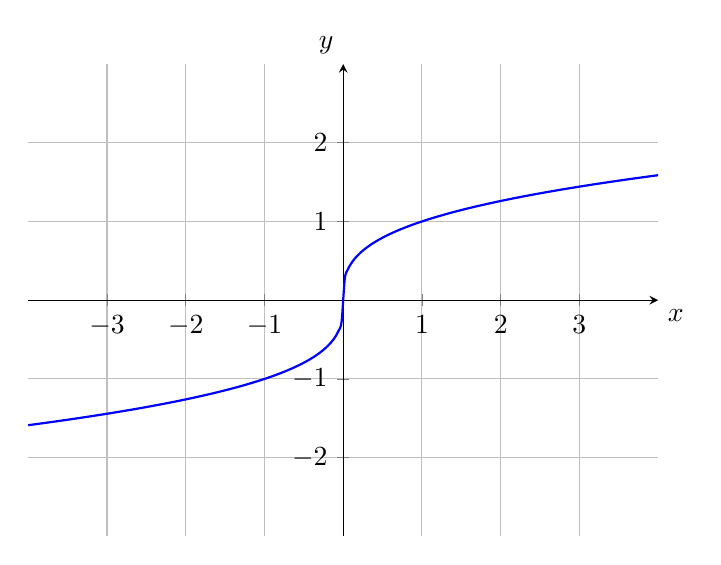
\begin{tikzpicture}
            \begin{axis}[
            x = 1cm, y = 1cm,
            xmin = -4, xmax = 4,
            ymin = -3, ymax = 3,
            axis lines = center,
            xtick={-3,-2,...,3},
            ytick={-2,-1,...,2},
            xlabel={$x$},
            ylabel={$y$},
            xlabel style={below right},
            ylabel style={above left},
            grid=both]
            \addplot[
                domain = -4:4,
                samples = 200,
                smooth,
                thick,
                blue,
            ] {sign(x) * abs(x)^(1/3)};
            \end{axis}
        \end{tikzpicture}
    \end{tabular}
\end{description}
\subsubsection{Exponentialfunktionen} $$f : \mathbb{R} \longrightarrow \mathbb{R}^+,\ x \longmapsto b^x \ | b \in \mathbb{R}^+ \setminus \lbrace 1 \rbrace$$
\begin{tabular}[t]{cc}
    $f : \mathbb{R} \longrightarrow \mathbb{R}^+,\ x \longmapsto 2^x$ & $f*^{-1} : \mathbb{R}^+ \longrightarrow \mathbb{R},\ x \longmapsto \log_2(x)$ \\
    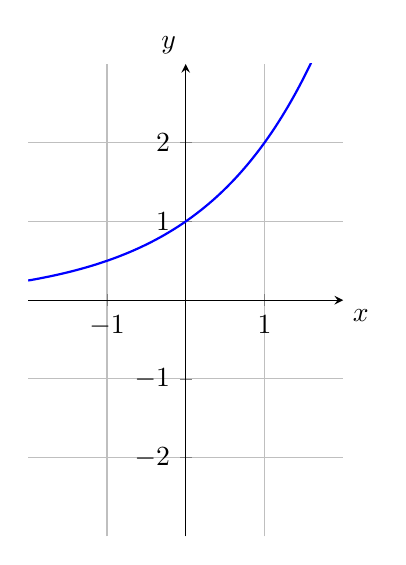
\begin{tikzpicture}
        \begin{axis}[
        x = 1cm, y = 1cm,
        xmin = -2, xmax = 2,
        ymin = -3, ymax = 3,
        axis lines = center,
        xtick={-1,0,...,1},
        ytick={-2,-1,...,2},
        xlabel={$x$},
        ylabel={$y$},
        xlabel style={below right},
        ylabel style={above left},
        grid=both]
        \addplot[
            domain = -2:2,
            samples = 200,
            smooth,
            thick,
            blue,
        ] {2^x};
        \end{axis}
    \end{tikzpicture}                                        &
    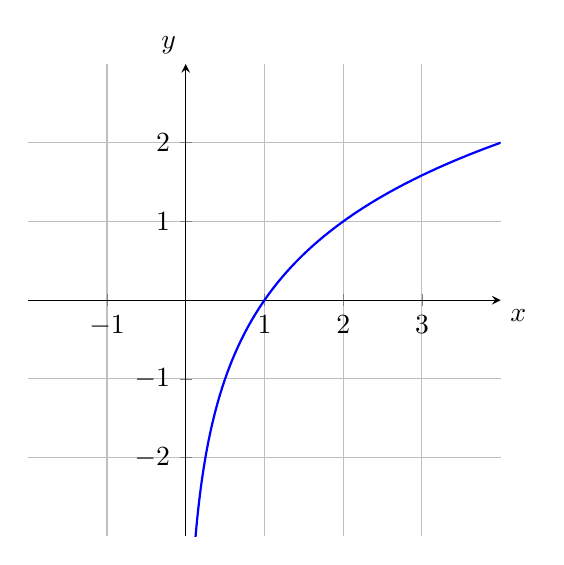
\begin{tikzpicture}
        \begin{axis}[
        x = 1cm, y = 1cm,
        xmin = -2, xmax = 4,
        ymin = -3, ymax = 3,
        axis lines = center,
        xtick={-1,0,...,3},
        ytick={-2,-1,...,2},
        xlabel={$x$},
        ylabel={$y$},
        xlabel style={below right},
        ylabel style={above left},
        grid=both]
        \addplot[
            domain = -0.01:4,
            samples = 200,
            smooth,
            thick,
            blue,
        ] {ln(x)/ln(2)};
        \end{axis}
    \end{tikzpicture}
\end{tabular}
